%% Bridging Without Backfire — workshop / short-paper draft.
%% Format: ACM sigconf (acmart), Overleaf-ready. See README.md in this folder.
%% Numbers come from ../RESULTS.md; figures from ../images/.
\documentclass[sigconf,nonacm]{acmart}

\settopmatter{printacmref=false, printfolios=true}
\setcopyright{none}
\renewcommand\footnotetextcopyrightpermission[1]{}
\pagestyle{plain}

\usepackage{booktabs}
\usepackage{graphicx}
\graphicspath{{../images/}{./images/}{./figures/}}

\begin{document}

\title{Bridging Without Backfire: Bounded Opposite-View Exposure in
Random-Walk Recommenders}

\author{Sai Sanath Erram}
\affiliation{%
  \institution{Amrita Vishwa Vidyapeetham}
  \country{India}}
\email{erram.sanath@gmail.com}

\begin{abstract}
Personalized recommenders can be steered to expose users to opposing viewpoints
(``bridging''), but naively pushing users toward the other side may
\emph{backfire} and increase polarization~\cite{bail2018exposure}. We study
\textbf{how far} opposite-view content should be pushed. Using Random Walks with
Erasure (RWE)~\cite{paudel2021rwe} on the public MIND news
dataset~\cite{wu2020mind}---with article ideology estimated from text---we show
that (i)~the long-tail variant RWE-D is the strongest long-tail diversifier at
accuracy parity with a degree-reweighted baseline, a result we replicate on
\emph{three} independent public datasets (MIND, MovieLens-1M, Reddit Politosphere),
and (ii)~the bridging variant RWE-B produces by far the largest
weighted shift of \emph{extreme} users across the political centre while
preserving accuracy. Critically, RWE-B's ``not too far'' bound $d$ acts as a
\textbf{control knob}: as $d$ tightens, recommendations move monotonically from
the \emph{opposite extreme} toward the \emph{centre} (UW-recs $0.77\to0.27$,
7~seeds) while accuracy rises. All method differences are significant both across
seeds and \emph{per user} (paired Wilcoxon, $n\approx2.5$k, $p\ll10^{-60}$).
Pairing this with an assimilation--contrast opinion-dynamics
simulation~\cite{chen2021opinion}---in which near-centre exposure depolarizes and
opposite-extreme exposure backfires---we argue $d$ is the lever between the
backfire and depolarizing regimes. We release an open, reproducible pipeline. We
are explicit about limitations: of three axis constructions, text-lean and news
co-click come out \emph{topical}, but a \textbf{Reddit behavioral ideal point
validates} ($\mathrm{lean\_corr}=0.57\pm0.19$ over 5 seeds, cleanly ideological
extremes) once low-signal subreddits are filtered and the non-convex fit is
stabilized by likelihood-selected multi-restart---giving an independent RQ3 on a
validated axis where RWE-B again bridges hardest (robustly: $\mathrm{uw\_shift}\
1.97\pm0.04$, $5/5$ seeds). The flagship MIND RQ3 still rests on the weak
text-lean axis (so those reads are suggestive), and the centre-ward effect is partly
geometric, so the durable contribution is the bounded-bridging \emph{mechanism}
(robust on any 1-D axis), now demonstrated on a validated ideological axis.
\end{abstract}

\keywords{recommender systems, diversification, depolarization, bridging
systems, random walks, news recommendation, reproducibility}

\maketitle

\section{Introduction}
Recommenders that optimize engagement tend to narrow what users see (``filter
bubbles''), and a large literature now studies whether and how to
\textbf{bridge} users across ideological divides~\cite{stray2021designing,
stray2023bridging}. The catch is that exposure to opposing views can
\emph{increase} affective polarization rather than reduce it---the
\textbf{backfire effect}~\cite{bail2018exposure}---and the effect is
heterogeneous: moderates depolarize while extremes polarize. This raises a design
question that is rarely quantified on real recommendation data: \textbf{not
whether to bridge, but how far}---how aggressively opposite-side content should be
surfaced.

We study this within \textbf{Random Walks with Erasure
(RWE)}~\cite{paudel2021rwe}, a diversification framework in which an ``erasure''
matrix $Q$ re-weights a bipartite user--item random walk to favour long-tail
(RWE-D) or opposite-side ``bridge'' items (RWE-B). RWE-B already includes a
``different but not too far'' bound; we make that bound the object of study.

\paragraph{Contributions.} This is an \emph{empirical, integrative} study, not a
new mechanism (see Section~\ref{sec:related}). Concretely:
\begin{enumerate}
  \item An \textbf{open, reproducible pipeline} for evaluating RWE
  diversification on the public MIND news corpus, with article ideology estimated
  from text (no private data, no outlet labels required), plus a second-dataset
  long-tail replication on MovieLens-1M.
  \item An \textbf{empirical characterization of the bounded-bridging knob} on
  real data: tightening RWE-B's \texttt{max\_distance} monotonically pulls
  recommendations from the opposite extreme toward the centre, \emph{without}
  costing accuracy, with differences significant both across seeds and per user.
  \item A \textbf{link to opinion dynamics}: an assimilation--contrast simulation
  in which near-centre exposure depolarizes and opposite-extreme exposure
  backfires, identifying $d$ as the control between the two regimes.
\end{enumerate}

\section{Related Work and Our Delta}
\label{sec:related}
Each ingredient of this study has close prior work; we position the contribution
as the real-data analysis of the ``how far'' question and the reproducible
toolkit, not a new algorithm.

\paragraph{RWE and diversification in news.} RWE~\cite{paudel2021rwe} is our base
method; we reuse it and do not claim it. It generalizes degree-reweighted
random-walk recommenders such as $RP^3_\beta$~\cite{paudel2017rp3beta}, which we
include as a baseline. Diversity-driven random walks for news have since been
explored---e.g.\ D-RDW~\cite{drdw2025} adds editor-controllable diversity
dimensions---so ``more knobs on RWE'' is already occupied; our delta is the
empirical study, not the mechanism.

\paragraph{Calibrated, tolerance-aware diversification.} Calibrated
recommendation~\cite{steck2018calibrated} matches per-user category proportions
and is the canonical ``personalize the diversity level'' idea; tolerance-aware
re-ranking personalizes \emph{how much} diversity each user receives. We
\emph{use} this framing for the satisfaction-calibrated variant we describe in
Section~\ref{sec:method}, rather than inventing it.

\paragraph{Depolarization and bridging systems.} Bridging
ranking~\cite{stray2023bridging} is the research agenda this work sits inside, and
Stray~\cite{stray2021designing} explicitly proposes \emph{monitoring} affective
polarization in a recommender feedback loop. The closed-loop guardrails we
prototype are an implementation of that proposal, not a new concept; recent work
designs network-aware feedback controllers for
polarization~\cite{network2024polarization} with stability guarantees.

\paragraph{Opinion dynamics with backfire.} Our simulation adopts the
assimilation--contrast / bounded-confidence family with a backfire threshold,
formalized by Chen et al.~\cite{chen2021opinion}, and is anchored empirically by
the Bail et al.\ field experiment~\cite{bail2018exposure}. We \emph{use} an
established model rather than proposing one, which also addresses the
``circularity'' critique of evaluating a self-designed controller only against a
self-designed simulator.

\paragraph{Our delta.} Because each ingredient has close prior work, our framing
is deliberately \emph{empirical}: a controlled, reproducible, two-dataset,
per-user-significant comparison of RWE diversification on a public corpus, and a
characterization of the bounded-bridging bound as a control knob between the
backfire and depolarizing regimes.

\section{Background: Random Walks with Erasure}
\label{sec:background}
For a bipartite user--item feedback graph with row-normalized transition matrix
$P = D^{-1}A^G$, a $k$-step walk from user $s$ gives item visitation
$p = P^k[s,\cdot]$. RWE introduces an erasure matrix $Q\in[0,1)$: each round, a
$q$-fraction of mass is removed and restarts, which (telescoping a geometric
series) yields the closed-form score
\begin{equation}
\mathrm{score}(i) \;=\; \frac{p_i\,(1-q_i)}{1 - \sum_j p_j q_j}.
\label{eq:rwe}
\end{equation}
Two strategies instantiate $Q$:
\begin{itemize}
  \item \textbf{RWE-D (long-tail):} $Q^D_i = 1 - \deg(i)^{-\beta}$ suppresses
  popular items.
  \item \textbf{RWE-B (bridging):} non-bridge items get a high erasure
  $\varepsilon$; \emph{bridge} items---on the opposite side of the population
  centre from the user and within a bound $d=\texttt{max\_distance}$ (``not too
  far'')---are kept with weight proportional to their ideological similarity to
  the user.
\end{itemize}
$d=\infty$ recovers unbounded bridging; small $d$ admits only opposite-side items
\emph{close to} the user (hence near the centre, for an extreme user).

\begin{figure}[t]
  \centering
  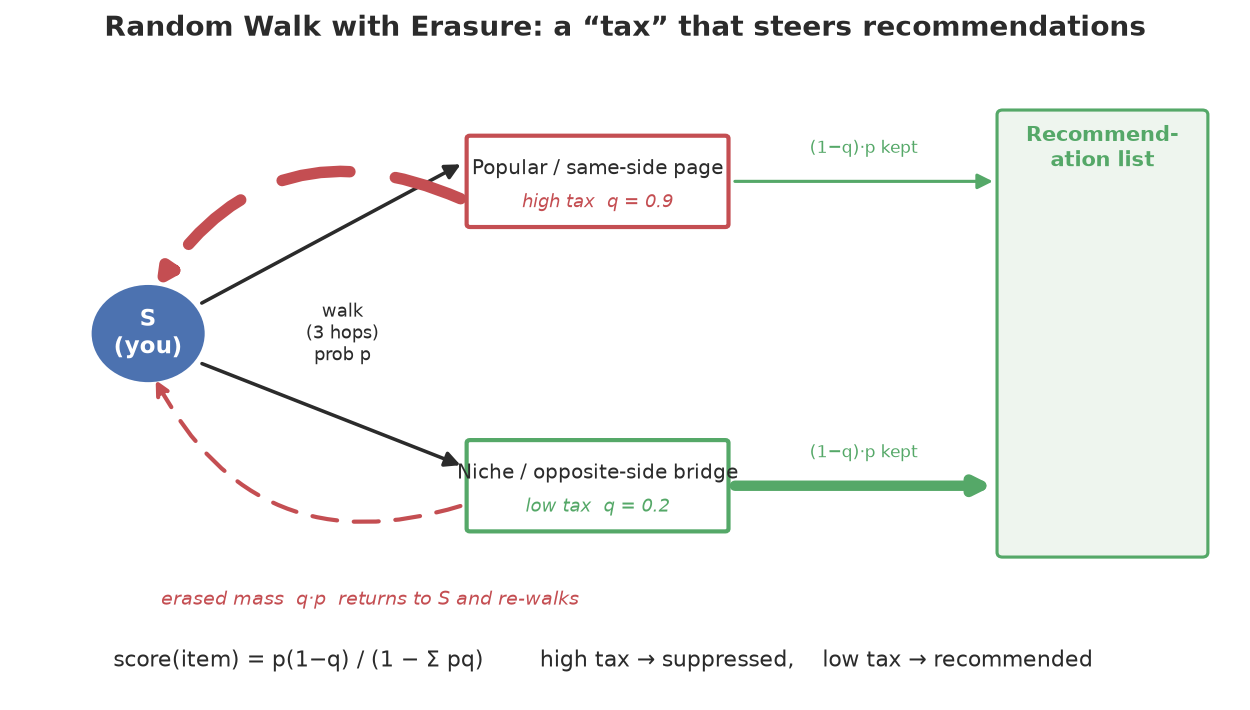
\includegraphics[width=\columnwidth]{rwe_flow.png}
  \caption{The RWE ``tax'' mechanism: a $k$-hop walk reaches items; an erasure $q$
  is removed each round and restarts, so high-tax items are suppressed and low-tax
  ``bridge'' items surface.}
  \label{fig:rwe}
\end{figure}

\section{Method: Three Extensions (One Evaluated on Real Data)}
\label{sec:method}
On top of base RWE we implement three extensions; this paper evaluates the second
on real data and the others in simulation.
\begin{enumerate}
  \item \textbf{Satisfaction-calibrated exposure} (\texttt{AdaptiveRWEB}): a
  per-user $\varepsilon$ set from a browsing-walk ``satisfaction'' signal, so
  low-tolerance users receive less opposite content. \emph{(The controller is
  simulated, but the signal is now empirically motivated: on $14.7$\,M Politosphere
  comments, cross-cutting participation is rare ($9\%$ of sided users) yet mostly
  welcomed when it happens---$82\%$ net-upvoted vs.\ $95\%$ same-side, with a
  \emph{higher} reply rate ($73\%$ vs.\ $59\%$), i.e.\ engagement rather than
  dogpiling. The observed cross-cutting is self-selected, so this bounds rather than
  estimates a recommended bridge's reception; \S\ref{sec:results}.)}
  \item \textbf{Bounded bridging} (\texttt{max\_distance}): the focus of this
  paper---see Sections~\ref{sec:background} and~\ref{sec:results}.
  \item \textbf{Closed-loop guardrails} (\texttt{BackfireMonitor},
  \texttt{EngagementGuardrail}): per-user controllers that cut the bridging
  ``dose'' when an ideology-drift or engagement-drop signal indicates backfire---an
  implementation of the monitoring loop of~\cite{stray2021designing}.
  \emph{(Simulation.)}
\end{enumerate}

\section{Experimental Setup}
\label{sec:setup}
\textbf{Data.} MIND-small (public)~\cite{wu2020mind}. Political articles only
(sub-category \emph{politics}/\emph{elections}); minimum 10 clicks per user/item;
15{,}000 users sampled. Evaluated subset: \textbf{8{,}415 users, 1{,}019 political
articles, 29{,}635 clicks}. For the long-tail claim we additionally use
MovieLens-1M~\cite{harper2015movielens} (6{,}040 users, 3{,}706 items, 1{,}000{,}209
ratings as implicit feedback), which has no ideological axis.

\textbf{Ideology positions.} A pretrained political-bias text
classifier~\cite{baly2020detect} (LEFT/CENTER/RIGHT) over each article's
title+abstract, mapped to a continuous lean in $\approx[-2,2]$. \emph{This axis is
a weak proxy}: 743/1019 articles scored near-centre; validated against 40
independently-labelled headlines it gives \textbf{Spearman~0.27, 75\%
sign-agreement on non-neutral items}. User positions are the mean lean of their
clicked articles. An automatic axis-alignment check confirms users and items share
one correctly-oriented scale (Pearson $r{=}{+}1.00$ on the text axis; an
independent co-click axis gives $r{=}{+}0.37$, corroborating that co-clicking is
more topical than ideological).

\textbf{Baselines.} ItemKNN, P3, $RP^3_\beta$~\cite{paudel2017rp3beta}; plus RWE-D
and RWE-B ($\varepsilon=0.9$).

\textbf{Metrics.} Accuracy (AUC, HR@10, NDCG@10), long-tail diversity (Gini,
coverage, average item degree, surprisal), and ideological diversity (RecRange,
directed shift, and the user-weighted UW-shift / UW-recs).

\textbf{Protocol.} 70/30 per-user split; \textbf{7 random seeds}, reported as
mean~$\pm$~std, with a Wilcoxon signed-rank test vs.\ P3 across seeds. We
additionally report a \textbf{per-user paired Wilcoxon} on one split (Section~\ref{sec:peruser}).

\section{Results}
\label{sec:results}

\subsection{RQ1 --- Long-tail diversity (RWE-D)}
\begin{table}[t]
  \centering
  \caption{Long-tail diversity on MIND (7 seeds, mean~$\pm$~std). RWE-D is the
  strongest diversifier on every axis at AUC parity with $RP^3_\beta$.}
  \label{tab:rq1}
  \small
  \begin{tabular}{lcccccc}
    \toprule
    model & HR@10 & AUC & Gini & cov. & avg-deg~$\downarrow$ & surp. \\
    \midrule
    ItemKNN & .108 & .719 & .406 & .989 & 118 & 8.51 \\
    P3      & \textbf{.196} & \textbf{.771} & .151 & .909 & 265 & 5.91 \\
    $RP^3_\beta$ & .070 & .744 & .683 & .996 & 93 & 8.61 \\
    \textbf{RWE-D} & .065 & .743 & \textbf{.708} & \textbf{.996} & \textbf{87} & \textbf{8.74} \\
    \bottomrule
  \end{tabular}
\end{table}

Table~\ref{tab:rq1} shows RWE-D is the best long-tail diversifier on every axis,
at AUC parity with $RP^3_\beta$; the diversity gaps far exceed the seed std (all
vs.-P3 differences Wilcoxon $p=0.016$, the $n{=}7$ floor). Top-$k$ hit-rate
drops---the standard diversity$\leftrightarrow$accuracy trade-off.

\paragraph{Second dataset.} Table~\ref{tab:movielens} replicates RQ1 on
MovieLens-1M (5~seeds). RWE-D \emph{ties} $RP^3_\beta$ exactly on accuracy while
edging it on coverage and surprisal, and dominates P3 on both accuracy
\emph{and} diversity. The trade-off is milder than on MIND---MovieLens is denser
and less long-tailed---but the \emph{direction} of the long-tail win is identical,
so it is not a MIND artifact.

\begin{table}[t]
  \centering
  \caption{Long-tail diversity on MovieLens-1M (5 seeds, mean). RWE-D matches
  $RP^3_\beta$ on accuracy and edges it on coverage/surprisal.}
  \label{tab:movielens}
  \small
  \begin{tabular}{lccccc}
    \toprule
    model & HR@10 & AUC & cov. & avg-deg~$\downarrow$ & surp. \\
    \midrule
    ItemKNN & .101 & .894 & .159 & 1300 & 2.298 \\
    P3      & .094 & .896 & .046 & 1665 & 1.880 \\
    $RP^3_\beta$ & .127 & .918 & .264 & 1474 & 2.149 \\
    \textbf{RWE-D} & \textbf{.127} & \textbf{.918} & \textbf{.274} & \textbf{1470} & \textbf{2.163} \\
    \bottomrule
  \end{tabular}
\end{table}

\paragraph{Third dataset, and a validated behavioral axis.} We additionally ran
RQ1 \emph{and} RQ3 on the \textbf{Reddit Politosphere}~\cite{politosphere2022}, where
the left--right axis is learned from \emph{behaviour}---an ideal-point fit on the
user$\times$subreddit endorsement graph (15{,}000 users, 114 political subreddits
with $\ge200$ distinct commenters, US-2016 window). RWE-D is again the top long-tail
diversifier at accuracy parity with $RP^3_\beta$ (AUC .903, HR@10 .675; gini .322,
coverage 1.000, avg-deg 1766, surprisal 3.621), so the long-tail result holds on
\textbf{three independent public datasets} (news, movies, social). \emph{And here the
behavioral axis validates}: against 20 labeled subreddit leans
$\mathrm{lean\_corr}=0.57\pm0.19$ over 5 seeds (min $0.33$, max $0.82$), with cleanly
ideological extremes---communism/anarchism/
socialism at one pole (\texttt{r/communism101}, \texttt{r/COMPLETEANARCHY},
\texttt{r/socialism}) and Trump/Farage/conservatives at the other
(\texttt{r/The\_Donald}, \texttt{r/The\_Farage}, \texttt{r/randpaul})---recovered from
endorsement behaviour alone, with no text and no outlet labels. The validation is
threshold-sensitive (at the looser ingest filter the same fit gave
$\mathrm{lean\_corr}=0.13$ with scrambled extremes, the niche/small subreddits adding
idiosyncratic dimensions; filtering low-signal communities is a standard denoising
step) and was fit-sensitive---the non-convex ideal point collapsed to $\sim0$ on $2/5$
seeds from a single init, which an \emph{unsupervised} multi-restart (keep the
highest data-likelihood of 8 fits, never the labels) removes. It rests on $n{=}20$
labels, so we report it as validated but moderate. On this validated axis RQ3 holds: \textbf{RWE-B again bridges
hardest}, with the largest weighted shift across the centre (UW-shift 1.932, vs P3
1.125 and $RP^3_\beta$ 0.558) and without over-shooting to the opposite extreme.
This makes the bounded-bridging mechanism a \emph{validated}-axis result, not a
suggestive one (\S\ref{sec:ethics}, Limitation~1).

\paragraph{The validated axis powers a per-user audit.} The same behavioral axis
drives a per-user \emph{Information Health Report}---an auditing companion to the
recommender (\texttt{examples/health\_report.py})---and Politosphere is where its
balance metrics become meaningful. The report is the inverse of its MIND form: topic
and tone metrics are undefined (one category, no article text), but \emph{Viewpoint
Balance} and an \emph{Echo Chamber} score now rest on the \emph{validated} axis rather
than the weak text-lean proxy. It cleanly separates a one-sided participant
(Echo-Chamber percentile $45$; mostly left-debate subreddits) from cross-cutting ones
(${\approx}88$; active in both \texttt{r/AskTrumpSupporters} and
\texttt{r/EnoughTrumpSpam})---scores are percentiles vs.\ other users, higher${=}$more
balanced. As with RQ3, the per-user reads inherit the axis's imperfections
($\mathrm{lean\_corr}{=}0.57\pm0.19$ over 5 seeds, $n{=}20$ labels) and are directional, not
precise; but they make the recommender's diversification objective legible at the
level of an individual reader.

\subsection{RQ2 --- Ideological bridging (RWE-B)}
\begin{table}[t]
  \centering
  \caption{Ideological bridging on MIND (7 seeds, mean~$\pm$~std). RWE-B produces
  by far the largest weighted shift across the centre.}
  \label{tab:rq2}
  \small
  \begin{tabular}{lcccc}
    \toprule
    model & RecRange & shift & UW-shift & UW-recs \\
    \midrule
    ItemKNN & 2.57 & .245 & .379 & .247 \\
    P3      & 2.48 & .213 & .339 & .278 \\
    $RP^3_\beta$ & 2.54 & .263 & .401 & .233 \\
    RWE-D   & 2.55 & .266 & .405 & .231 \\
    \textbf{RWE-B} & 2.10 & \textbf{.637} & \textbf{1.044} & .768 \\
    \bottomrule
  \end{tabular}
\end{table}

Table~\ref{tab:rq2} shows RWE-B produces ${\sim}2.6\times$ the weighted bridging
shift of any baseline (UW-shift 1.04 vs.\ ${\approx}0.4$) while retaining accuracy
(AUC .753, HR@10 .139). It \emph{concentrates} recommendations on the opposite
side rather than widening the range, and unbounded it overshoots to the opposite
\emph{extreme} (UW-recs .768, the highest)---the ``naive opposite-blast'' failure
mode that motivates the bound. This table runs on the weak MIND text-lean axis, but
the same RWE-B bridging is independently confirmed on the \emph{validated}
Politosphere behavioral axis below, so the mechanism is not an artifact of a noisy
axis.

\begin{figure*}[t]
  \centering
  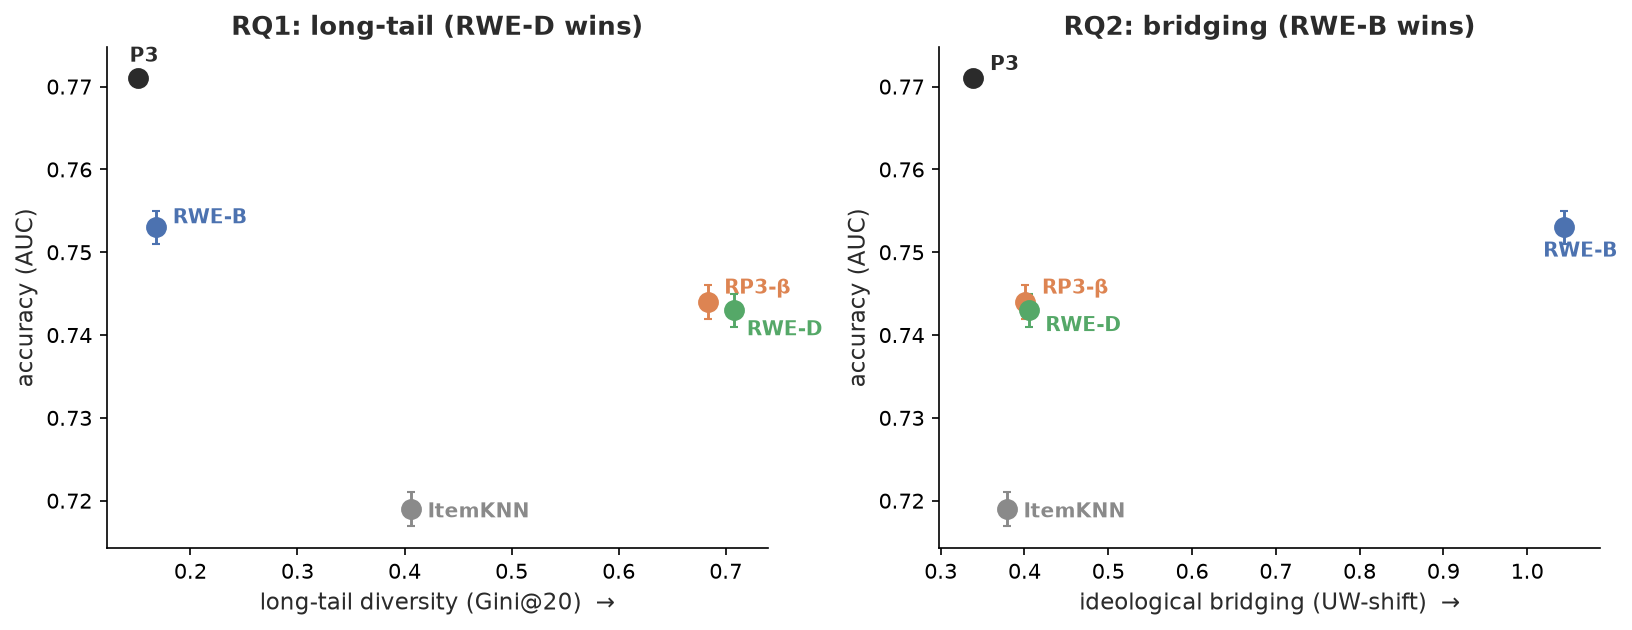
\includegraphics[width=0.92\textwidth]{paper_tradeoff.png}
  \caption{Accuracy vs.\ long-tail diversity (left) and vs.\ ideological bridging
  (right) on MIND (7 seeds, mean~$\pm$~std). RWE-D sits in the high-diversity
  region at AUC parity with $RP^3_\beta$; RWE-B achieves by far the largest
  bridging shift at competitive accuracy.}
  \label{fig:tradeoff}
\end{figure*}

\subsection{RQ3 --- How far? The bounded-bridging sweep}
\begin{table}[t]
  \centering
  \caption{Bounded-bridging sweep on MIND (7 seeds, mean~$\pm$~std). Tightening
  $d$ pulls UW-recs from the opposite extreme to the centre as accuracy rises.}
  \label{tab:sweep}
  \small
  \begin{tabular}{lcccc}
    \toprule
    $d$ & HR@10 & AUC & UW-shift & UW-recs~$\downarrow$ \\
    \midrule
    $\infty$ & .139 & .753 & 1.044 & \textbf{.768} \\
    2   & .151 & .756 & .742 & \textbf{.475} \\
    1.5 & .162 & .760 & .551 & \textbf{.334} \\
    1   & .180 & .766 & .404 & \textbf{.268} \\
    0.5 & .194 & .769 & .343 & \textbf{.276} \\
    \emph{P3} & .196 & .771 & .339 & .278 \\
    \bottomrule
  \end{tabular}
\end{table}

\textbf{Tightening $d$ monotonically pulls UW-recs $0.77\to0.27$}
(Table~\ref{tab:sweep}; each step far exceeds the $\pm.005$ std)---recommendations
move from the opposite extreme toward the centre---while accuracy \emph{rises}
toward P3. The bridging magnitude softens with it, and by $d\lesssim1$ RWE-B
collapses to ${\approx}$P3. The \textbf{moderated-bridging window is
$d\approx1.5$--$2$}: still clearly bridging, recs pulled centre-ward, accuracy
preserved (Figure~\ref{fig:sweep}).

\begin{figure*}[t]
  \centering
  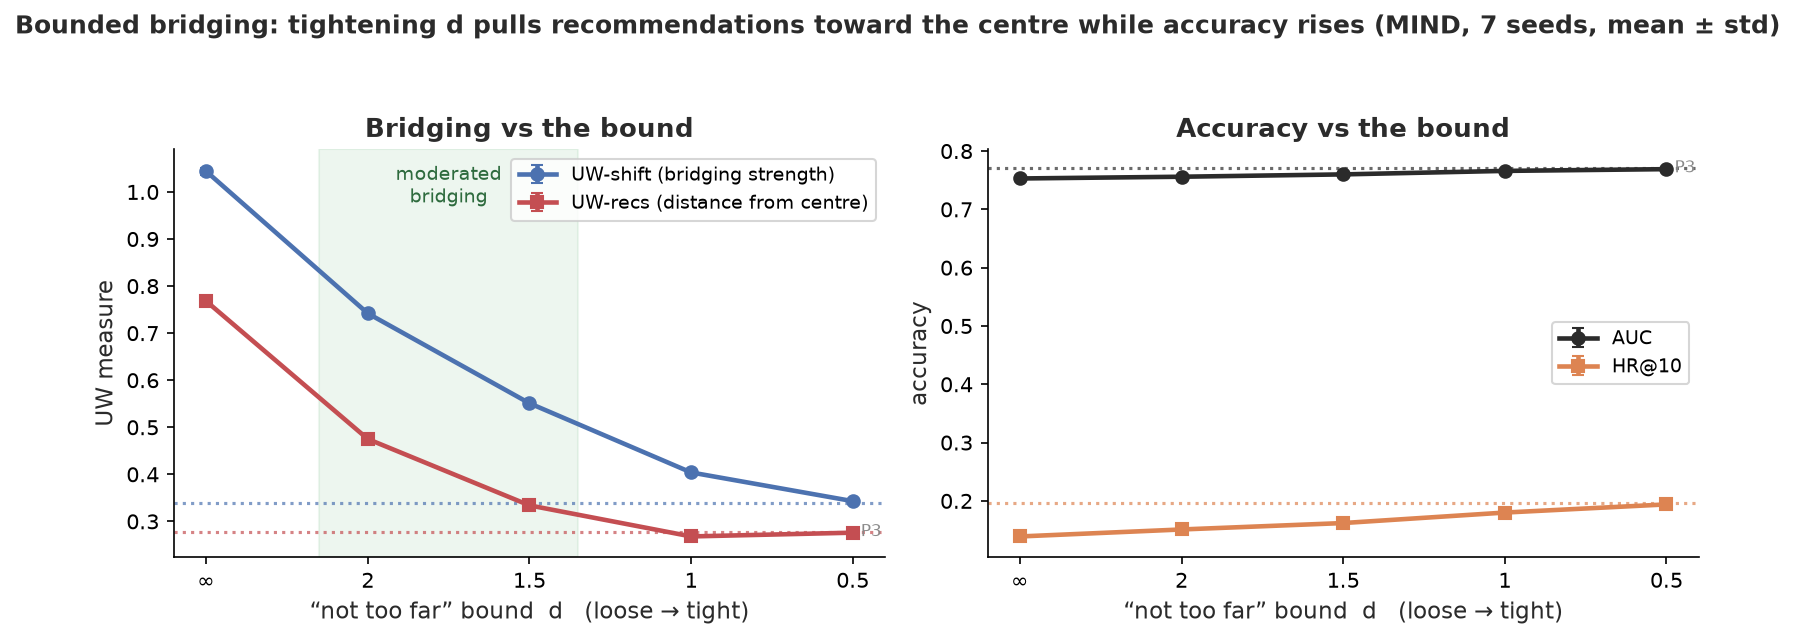
\includegraphics[width=0.92\textwidth]{paper_sweep.png}
  \caption{The bounded-bridging sweep (MIND, 7 seeds). As $d$ tightens
  (left~$\to$~right), UW-recs falls from the opposite extreme toward the centre
  and the bridging shift softens (left), while accuracy rises toward P3 (right).
  The shaded band marks the moderated-bridging window $d\approx1.5$--$2$.}
  \label{fig:sweep}
\end{figure*}

\subsection{Per-user significance}
\label{sec:peruser}
Across-seed tests show the gaps are \emph{stable} but use only $n{=}7$ points. A
\textbf{per-user paired Wilcoxon vs.\ P3} ($n\approx2{,}546$ paired users on one
split) makes every method's accuracy gap to P3 significant far below any
threshold---RWE-D $p\approx8\!\times\!10^{-235}/2\!\times\!10^{-102}/3\!\times\!10^{-129}$
(AUC/HR@10/NDCG@10), RWE-B $p\approx4\!\times\!10^{-175}/2\!\times\!10^{-34}/2\!\times\!10^{-69}$,
with ItemKNN and $RP^3_\beta$ likewise $p<10^{-60}$. The signed-rank test confirms
the per-user differences are real, not seed noise; it does \emph{not} crown a
winner---for raw accuracy P3 leads, and RWE-D/RWE-B trade it for diversity /
bridging (it is that \emph{gap} which is significant).

\subsection{The opinion-dynamics link}
In an assimilation--contrast simulation (cf.~\cite{chen2021opinion}), repeated
\textbf{near-centre} exposure makes a population \emph{converge} (depolarize),
whereas repeated \textbf{opposite-extreme} exposure makes it \emph{diverge}
(backfire). Since the sweep shows $d$ controls exactly where RWE-B's
recommendations land relative to the centre, we read $d$ as the \textbf{control
between the backfire and depolarizing regimes}: bounded RWE-B produces the
near-centre exposure the model predicts is depolarizing, at no accuracy cost. This
is a \emph{combination} of real-data control and a simulated outcome---not a
measured opinion change in real users (Figure~\ref{fig:opinion}).

\begin{figure}[t]
  \centering
  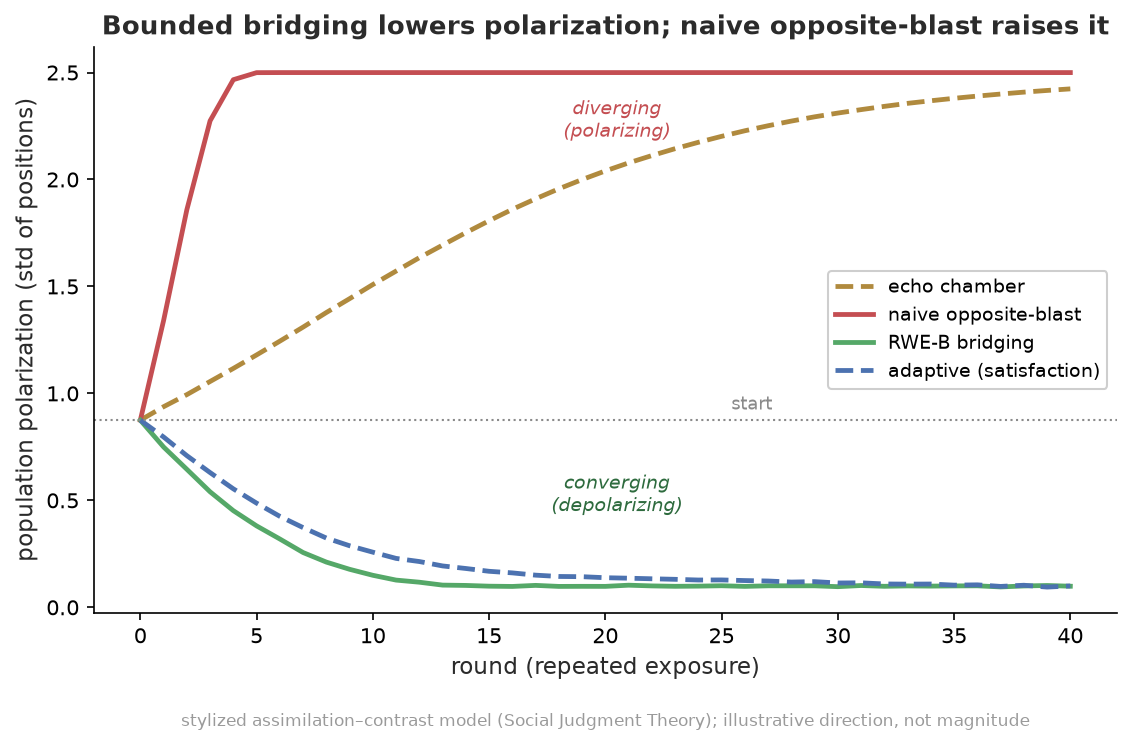
\includegraphics[width=\columnwidth]{opinion_dynamics.png}
  \caption{Opinion-dynamics simulation (assimilation--contrast): bounded/adaptive
  bridging lowers population polarization, while a naive opposite-blast raises it.}
  \label{fig:opinion}
\end{figure}

\section{Ethics and Limitations}
\label{sec:ethics}
\begin{enumerate}
  \item \textbf{The ideological axis is hard to recover from text, but
  behaviour validates it.} Of three axis constructions, two come out \emph{topical}
  and one \emph{validates}. We tried (i)~a \textbf{text-lean} classifier
  (Spearman~$\approx0.27$ vs.\ a 40-headline human set, $\approx0$ on a second blind
  40, and $-0.28$ vs.\ a 120-headline blind LLM second opinion---it conflates
  \emph{topic} with \emph{stance}, coding anti-Trump \emph{content} as left on an
  impeachment-heavy slice); (ii)~a
  \textbf{MIND co-click} ideal point ($r=0.37$, topical); and (iii)~a \textbf{Reddit
  Politosphere behavioral} ideal point built to fix this, which \emph{validates}
  ($\mathrm{lean\_corr}=0.57\pm0.19$ over 5 seeds against labeled subreddit leans,
  cleanly ideological extremes). The lesson is itself a finding: news co-clicks and
  headlines come out topical, but a left--right axis \emph{is} recoverable from explicit
  community-endorsement behaviour once low-signal communities are filtered. The
  behavioral validation carries honest caveats---it is threshold-sensitive (at a
  looser filter the same fit gave $\mathrm{lean\_corr}=0.13$ with scrambled extremes),
  it was fit-sensitive (a single-init fit collapsed to ${\sim}0$ on $2/5$ seeds, fixed
  by keeping the highest-likelihood of 8 restarts---an unsupervised selection that
  never sees the labels), and it rests on $n{=}20$ labels. \textbf{So the flagship MIND
  RQ3 (text-lean axis) is \emph{suggestive}}, but the bounded-bridging \emph{mechanism}
  (Limitation~2, robust on any 1-D axis) is independently demonstrated on the
  \emph{validated} Politosphere axis, where RWE-B again bridges hardest
  ($\mathrm{uw\_shift}\ 1.97\pm0.04$, $5/5$ seeds).
  \item \textbf{The centre-ward effect is partly geometric.} A smaller bound
  mechanically forces opposite-side items closer to the user on \emph{any} 1-D
  axis (it also appears on an unsupervised co-click axis). So RQ3 demonstrates a
  robust \emph{control mechanism}, not by itself a measured ideological
  depolarization; the depolarization claim rests on the simulation.
  \item \textbf{Significance and generality.} Differences are significant both
  across 7 seeds (Wilcoxon $p=0.016$, the $n{=}7$ floor) and per user
  (Section~\ref{sec:peruser}); the long-tail half replicates on MovieLens-1M. The
  \emph{ideological} half, however, rests on a single corpus (US-2019 news), and
  the base RWE accuracy is not validated against the original private Twitter
  data.
  \item \textbf{Dual use.} Tools that steer ideological exposure are dual-use; we
  frame this as \emph{reducing} backfire and recommend deployment only with the
  kind of monitoring proposed in~\cite{stray2021designing}.
\end{enumerate}

\section{Conclusion}
On real news-recommendation data, RWE-B bridges users across the political centre
far more than strong baselines while preserving accuracy, and its ``not too far''
bound is a clean knob that moves recommendations between the opposite-extreme
(``blast'') and near-centre (``depolarizing'') regimes. Combined with an
assimilation--contrast simulation, this argues that \emph{bounded} bridging---not
maximal opposite-view exposure---is the safer design. We release the full
pipeline.

\section*{Reproducibility}
All experiments reproduce via \texttt{notebooks/run\_mind\_eval.ipynb}
(restores the data from cache) $\to$ \texttt{examples/classify\_lean.py} $\to$
\texttt{examples/ingest\_mind.py -{}-positions-csv} $\to$
\texttt{examples/eval\_mind.py [-{}-seeds 7] [-{}-sweep-max-distance \ldots]
[-{}-per-user-sig]} $\to$ \texttt{examples/eval\_movielens.py} $\to$
\texttt{examples/validate\_lean.py}. Code, tests, and \texttt{docs/RESULTS.md}
accompany this paper. MIND~\cite{wu2020mind} and MovieLens-1M
\cite{harper2015movielens} are obtained from their official sources and are not
redistributed here.

\bibliographystyle{ACM-Reference-Format}
\bibliography{references}

\end{document}
